\chapter{Timeline}
\label{chap:plan}
% Work Plan

This final chapter of this report describes the timeline, considering both the work to date and the plan for the next two years of research.
While the previous chapter described the methodology and evaluation, here we describe when each part of the project is expected to be addressed.

\section{Work to date}
% until now: what has been done
% - initial experiments
% - formalisation and problem definition
% - data

During the first year several activities have been done, with the goal to find and formulate proper Research Questions and to prepare the execution of the proposal.


\subsection{Seed paper reproduction}
% Experiment 1
% why
We started by analysing the paper by~\citet{bountouridis2018explaining} which presents a methodology to analyse how much information overlaps between different similar documents, identifying points of information that are corroborated or omitted.
The implementation provided with the paper has been analysed and reproduced, to get a deep understanding of how it works.
The main limitations of the implementation\footnote{\url{https://github.com/dbountouridis/InCredible}} provided with the paper are:

\begin{itemize}
    \item just reproduces the second part (sentence-level cliques) and not the first one
    \item Their demo\footnote{\url{http://fairnews.ewi.tudelft.nl/InCredible/}} just shows one specific article as main and one specific clique (not very interesting)
    \item a lot of parameters are not specified
\end{itemize}

% how


% limitations
In addition to these problems, the model described is based on TF-IDF which is not as robust with changes on the linguistic surface (as we saw in the next experiment). --> this is the motivation for 5.1.2
And also, it uses the similarity between TF-IDF just with a threshold, modelling the graph and cliques as unweighted (the weights are just used to select the most appropriate clique during their creation).

% role of this experiment
This experiment helped seeing the limitation of this type of work, that belongs to the second area of research evidenced in the Literature Review (\ref{sec:lit_relationships}. This paper provides a great way to analyse the overlap between articles and extracts pieces that have been omitted or that are corroborated, but does not investigate further in the reason behind the selection of what to include or not. This lead into researching more into the framing analysis. 



\subsection{Similarity models analysis}
% Experiment 2
After finding and exploring more advanced methods to find the similarity between texts by using language models, we experimented on how to use these methods.
% why?

% how?
Specifically on the sentence level, we experimented to see how the different methods were able to pick similar sentences, by setting up a small benchmark. The task was to find the most similar pairs of sentences coming from selected pairs of news articles which cover the same event (selection done manually, by considering three constraints: \textit{i)} describing the same event \textit{ii)} from different news outlets, \textit{iii)} published the same day).
Each model would extract the most similar 10 pairs, and we compared the results obtained qualitatively.

The selected models used in the benchmark are the following:
\begin{itemize}
    \item \textbf{TF-IDF}: with a feature size of 2000, preprocessing consists of lowercasing and tokenizing
    \item \textbf{GloVe-average}: considering GloVe (Which???) word embeddings, and doing an average of the vectors over the sentence
    \item \textbf{BERT}: using the embeddings provided by BERT~\cite{devlin2018bert} pre-trained on ???
    \item \textbf{USE}: using embeddings coming from Universal Sentence Encoder~\cite{cer2018universal}
\end{itemize}
The representations from these models have been used together with the cosine similarity.

For each pair of sentences that was provided by any of the models, we listed by manual analysis which differences were contained, by saying if some details were added or removed, or if different words were used.


\begin{figure}[!htb]
    \centering
    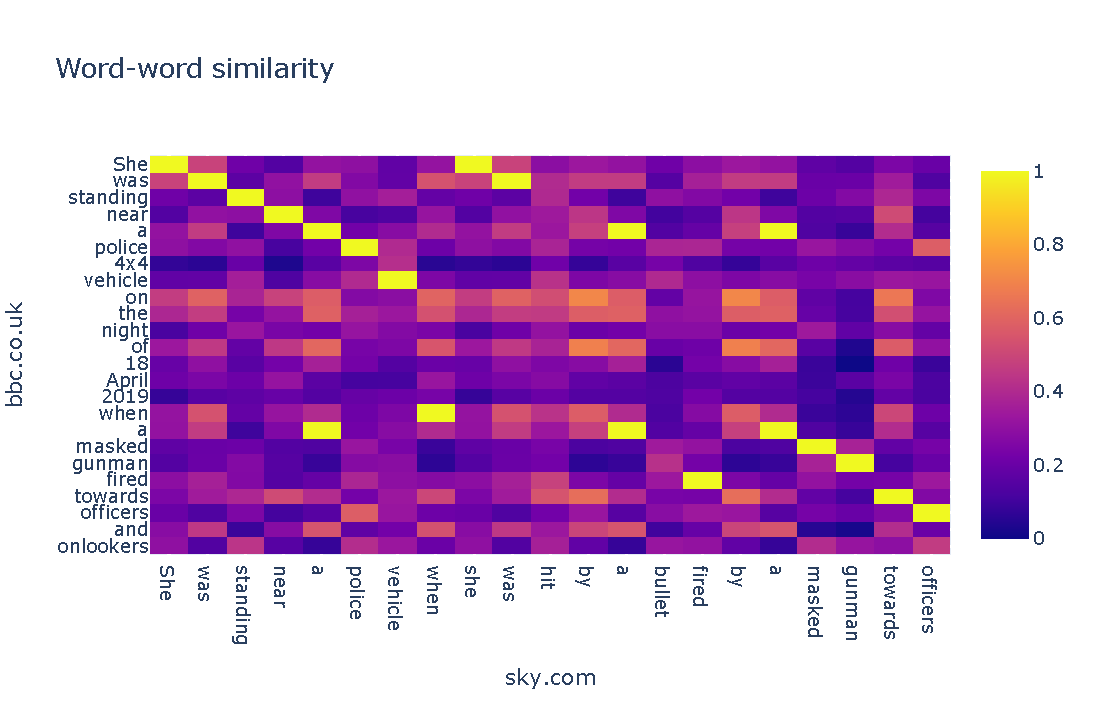
\includegraphics[width=\linewidth]{figures/lyra.pdf}
    \caption{Caption}
    \label{fig:lyra}
\end{figure}

An example can be seen in figure~\ref{fig:lyra} that shows a sentence from BBC and one from Sky, where the differences are the following:

\begin{itemize}
    \item the detail ``4x4'' just appears on the BBC article
    \item the detail ``on the night of 18 April 2019'' just appears on the BBC article
    \item Active vs passive sentence ``a masked gunman fired'' vs ``she was hit by a bullet fired by a masked gunman''
    \item the detail ``a bullet'' just appears in the Sky article
    \item ``Towards officers and onlookers'' vs ``towards officers'': in the second, the target of the gunman are just officers
\end{itemize}

With this kind of information on the types and magnitude of changes contained in the sentences, we can get a qualitative idea of how the different models say that two sentences are similar.


% Observations
The observations that we have for the TF-IDF model is that
Feature size changes a lot the results
Requires to be computed on a set of documents all together (which also changes which features are selected), not possible to encode an additional document without changing the representation of the already encoded documents
Pre-processing affects the results: if we don’t add a lemmatization step to the pipeline, it is sufficient to change the verb tense to have a different term.
Given these limitations, we find that sentences that are very similar in the meaning but have some differences in the linguistic surface see a drop in their similarity.

GloVe-average
To get the document-level or sentence level: average word vector for sentences and documents. This choice has been implemented by SpaCy https://spacy.io/usage/vectors-similarity , but has many negative aspects (e.g. “Luke hates John” == “John hates Luke”) 

BERT
The values provided are very similar. This per-se is not a problem if some geometric properties are valid (ordering, proportions)


Then we discovered STS benchmark

% role of this experiment
What this means for us:
- we need to use a similarity resistant to changes in the linguistic surface
- we need a measure that is able to represent well the different levels of similarity
- we must be able to switch the model used easily, in case new public benchmarks for STS show a different winner. (example XLNet~\cite{yang2019xlnet}


\subsection{Sentence clustering}
% Experiment 3

% why

% how
hierarchical clustering: example with diagram
\begin{figure}[!htb]
    \centering
    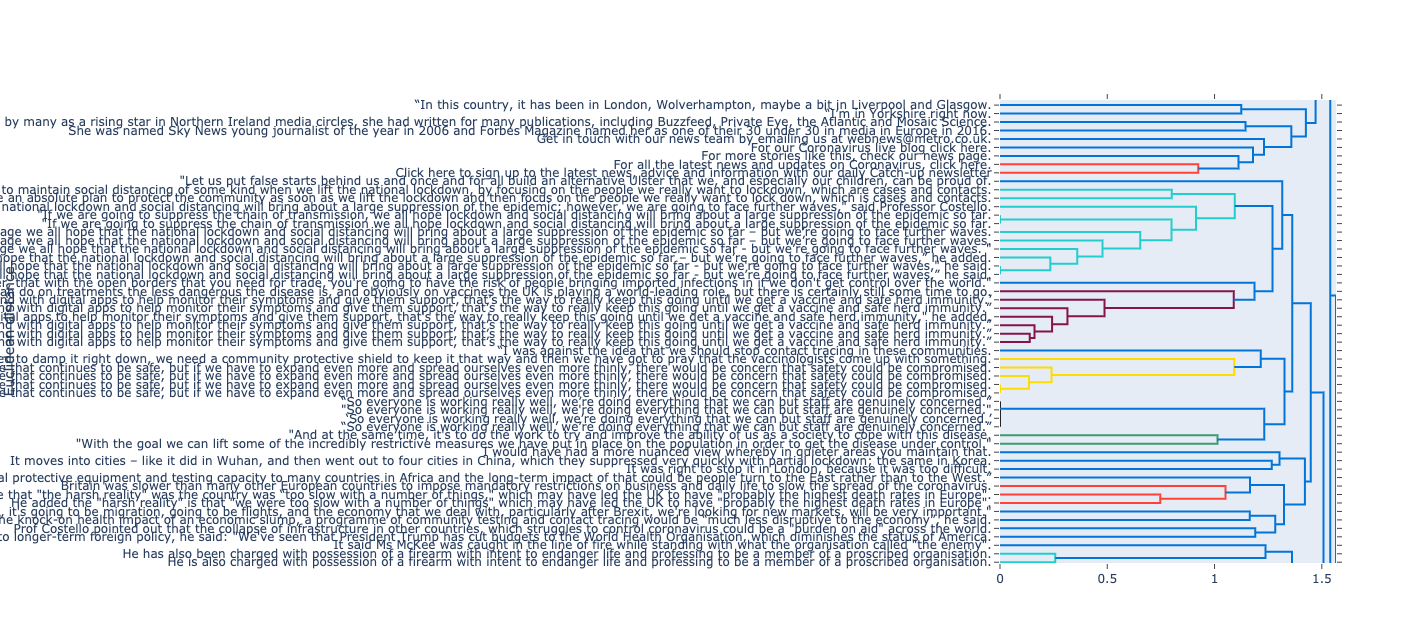
\includegraphics[width=\linewidth]{figures/dendrogram.png}
    \caption{Caption}
    \label{fig:my_label}
\end{figure}

sentence clusters: example with figure


% role of this experiment

\subsection{Data collection}
% why
We also started the \emph{data collection}, that has been done since the first steps on this projects.
The data that we are interested in belongs to different natures.
A wide set of articles is needed, so some datasets of news articles have been retrieved.
But also specific data that contains articles grouped by stories (document clustered) is very important to have, in order to have:
- a gold standard for document clustering experiments
- a solid starting point to analyse differences between articles that talk about the same events.

% how
We have collected the following:
- allnews
- allsides
- google news (more than 500k articles)

% role of this

\subsection{Formalisation and dissemination}
Then the second task is the \emph{formalisation and definition} of the approach presented in Chapter~\ref{chap:proposal}.
From how to connect the different pieces together
And a position paper has been submitted, accepted and presented at a workshop on narrative analysis (Text2Story at ECIR) in April.
This position paper focused on describing the gap and the proposed cross-article signals that would show differences in how stories are narrated.

Presentations:
- KMi
- Text2Story
- OU Poster Competition
- CRC PhD conference






\section{Plan}

realistic
clearly stated milestones
dependencies explicit
contingency planning – risks identified
timeline – dates
resources
skills
pretty presentation

GANTT chart
\begin{figure}[!htb]
    \centering
        \begin{ganttchart}[
            y unit title=1cm,
            y unit chart=1cm,
            vgrid,
            hgrid,
            time slot format=isodate-yearmonth,
            time slot unit=month,
            title/.append style={draw=none, fill=barblue},
            title label font=\sffamily\bfseries\color{white},
            title label node/.append style={below=-1.6ex},
            title left shift=.05,
            title right shift=-.05,
            title height=1,
            bar/.append style={draw=none, fill=groupblue},
            bar height=.6,
            bar label font=\normalsize\color{black!50},
            group right shift=0,
            group top shift=.6,
            group height=.3,
            group peaks height=.2,
            bar incomplete/.append style={fill=green}
       ]{2020-07}{2022-09}
       \gantttitlecalendar{year, month}\\
        %   \ganttbar[
        %     progress=100,
        %     bar progress label font=\small\color{barblue},
        %     bar progress label node/.append style={right=4pt},
        %     bar label font=\normalsize\color{barblue},
        %     name=pp
        %   ]{Preliminary Project}{2020-09}{2020-12} \\
        % \ganttset{progress label text={}, link/.style={black, -to}}
        \ganttgroup{Pipeline}{2020-07}{2020-12} \\
            \ganttbar[progress=20, name=T0]{Implementation}{2020-07}{2020-12} \\
            % \ganttlinkedbar[progress=0]{Task B}{2021-07}{2021-12} \\
        \ganttgroup{RQ1}{2020-07}{2021-05} \\
            \ganttbar[progress=15, name=T11]{RQ1.1: Hypothesis}{2020-07}{2020-09} \\
            \ganttlinkedbar[progress=0]{RQ1.1: User study}{2020-10}{2020-10} \\
            \ganttlinkedbar[progress=0]{RQ1.1: Analysis}{2020-11}{2020-12} \\
            % \ganttbar[progress=0]{RQ1.2: Hypothesis}{2020-07}{2020-12} \\
            \ganttlinkedbar[progress=0,name=T12]{RQ1.2: User study}{2021-01}{2021-01}
            \ganttlink[link mid=.4]{T0}{T12}\\
            \ganttbar[progress=0]{RQ1.2: Analysis}{2021-02}{2021-03} \\
        \ganttgroup{RQ2}{2021-03}{2021-12} \\
          \ganttbar[progress=0,name=T21]{RQ2.1: Implementation}{2021-03}{2021-05}
          \ganttlink[link mid=.4]{T0}{T21}\\
            \ganttlinkedbar[progress=0]{RQ2.1: Analysis}{2021-05}{2021-06} \\
            % \ganttbar[progress=0]{RQ1.2: Hypothesis}{2020-07}{2020-12} \\
            \ganttbar[progress=0,name=T12]{RQ1.2: Implementation}{2021-07}{2021-09}\\
            \ganttlinkedbar[progress=0]{RQ1.2: Analysis}{2021-09}{2021-10} \\
        \ganttgroup{Thesis}{2022-03}{2022-09} \\
          \ganttbar[progress=0]{Writing}{2022-03}{2022-09}
    \end{ganttchart}
    \caption{Gantt chart}
    \label{fig:gantt}
\end{figure}

